\documentclass[border=0pt]{standalone}
\usepackage{mathptmx}
\usepackage{tikz}
\usepackage{pgfplots}
\pgfplotsset{compat=1.17}
\definecolor{cvis}{HTML}{2F6DB5}\definecolor{crule}{HTML}{D27A1E}
\definecolor{cfuse}{HTML}{2E8B57}\definecolor{cbad}{HTML}{C0392B}\definecolor{cink}{HTML}{2B2B2B}
\begin{document}
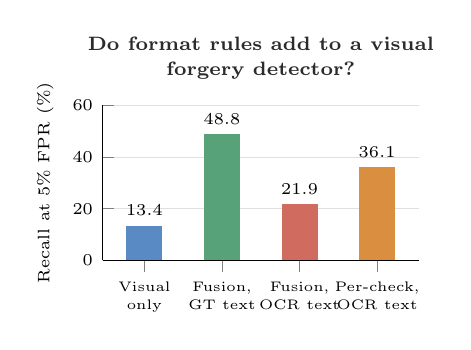
\begin{tikzpicture}

\begin{axis}[at={(0.85cm,0.75cm)}, anchor=south west, width=5.6cm, height=3.55cm, scale only axis=false,
  ybar, bar width=13pt, bar shift=0pt, ymin=0, ymax=60, ytick={0,20,40,60},
  symbolic x coords={V,G,O,P}, xtick={V,G,O,P},
  title={Do format rules add to a visual\\forgery detector?}, title style={font=\fontsize{7.5}{9}\selectfont\bfseries, text=cink, align=center},
  xticklabels={Visual\\only, {Fusion,\\GT text}, {Fusion,\\OCR text}, {Per-check,\\OCR text}},
  xticklabel style={font=\fontsize{5.5}{6.5}\selectfont, align=center},
  yticklabel style={font=\fontsize{6}{7}\selectfont},
  ylabel={Recall at 5\% FPR (\%)}, ylabel style={font=\fontsize{6}{7}\selectfont},
  axis lines*=left, ymajorgrids, grid style={black!12},
  nodes near coords, nodes near coords style={font=\fontsize{6.5}{7}\selectfont\bfseries},
  every axis plot/.append style={draw=none}, enlarge x limits=0.18]
\addplot[fill=cvis!80] coordinates {(V,13.4)};
\addplot[fill=cfuse!80] coordinates {(G,48.8)};
\addplot[fill=cbad!75] coordinates {(O,21.9)};
\addplot[fill=crule!85] coordinates {(P,36.1)};
\end{axis}
\end{tikzpicture}
\end{document}
